\chapter{Wprowadzenie do algorytmów percepcji głębi}\label{chap:2_wprowadzenie_do_algorytmów_percepcji_głębi}

\section{Paradygmaty uczenia}
Podstawową metodą uczenia algorytmów percepcji głębi jest uczenie nadzorowane. W tejże metodzie do nauki estymacji mapy głębi wykorzystywana jest struktura scen z obrazów określanych jako Ground truth\footnote{Dane rzeczywiste uzyskane za pomocą technologii rejestrowania obrazów 3D.}. Pozyskanie tych obrazów często bywa kosztowne i problematyczne, skąd wyniknęła potrzeba uczenia algorytmów przy użyciu zmniejszonej ilości danych rzeczywistych tudzież ich całkowitym braku\footnote{Wówczas mówimy o rekonstrukcji mapy głębi.}. W ramach usystematyzowania wiedzy następujący podrozdział skupi się zatem na zebraniu i sklasyfikowaniu paradygmatów uczenia algorytmów percepcji głębi.

\subsection{Uczenie nadzorowane}
Ta najczęściej obecnie stosowana metoda uczenia sieci neuronowych zakłada posiadanie odpowiednio przygotowanych danych wejściowych oraz odpowiadających im danych wyjściowych. Wówczas celem nauki jest zminimalizowanie wartości odpowiednio sporządzonej funkcji straty, której argumentami są wartości zmierzone i estymowane. Wybór wspomnianej funkcji zależy od charakterystyki rozwiązywanego problemu. W przypadku percepcji głębi najczęściej stosowaną funkcją straty jest błąd średniokwadratowy (MSE od ang. mean square error):
\begin{equation} \label{eq:1}
MSE = \frac{1}{n} \sum_{t=1}^{n} (d_i^* - d_i)
\end{equation}
gdzie \( d_i^* \) to wartość predykcji a \( d_i \) to wartość zmierzona.
Rysunek \ref{fig:uczenie-nadzorowane} przedstawia poglądowy schemat uczenia nadzorowanego.
\begin{figure}[H]
    \centering
    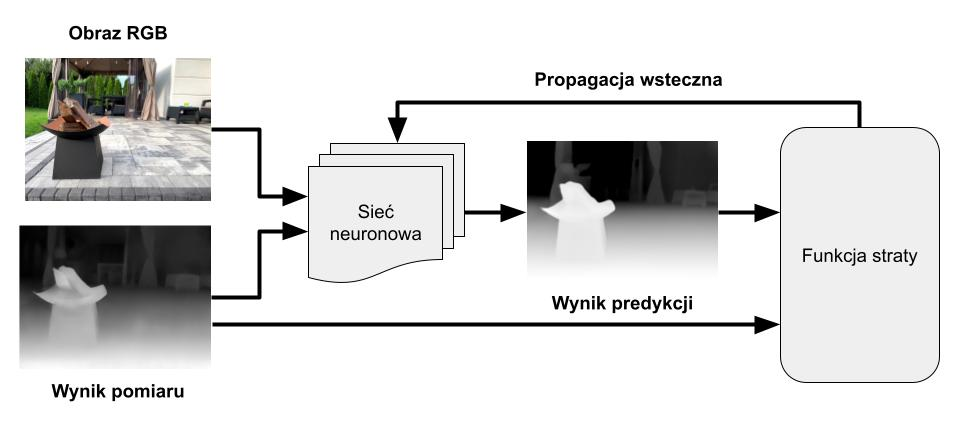
\includegraphics[width=0.85\textwidth]{2.jpg}
    \caption{Poglądowy model uczenia nadzorowanego. Wejścia stanowią obraz RGB oraz pomiary głębi a wynikiem jest predykcja mapy głębi.}
    \label{fig:uczenie-nadzorowane}
\end{figure}

\subsection{Uczenie nienadzorowane}
Z powodu potrzeby uniknięcia kosztownego procesu przygotowania danych na potrzeby uczenia nadzorowanego, rozwijana jest metoda uczenia nienadzorowanego. Algorytmy wykorzystujące tę metodę nauczane są zwykle przy pomocy zdecydowanie prostszych danych - par fotografii RGB lub nagrań wideo, czyli w uproszczeniu sekwencji fotografii RGB. Dane te przetwarzane są za pomocą funkcji, których zadaniem jest określenie głębi sceny przedstawionej na zdjęciu na podstawie zmian w perspektywie pomiędzy poszczególnymi kadrami. W ten sposób przygotowany zestaw wykorzystywany jest do nauki algorytmu podobnie jak w przypadku uczenia nadzorowanego. Na rys. \ref{fig:uczenie-nienadzorowane} znajduje się poglądowy schemat uczenia nienadzorowanego.
\begin{figure}[H]
    \centering
    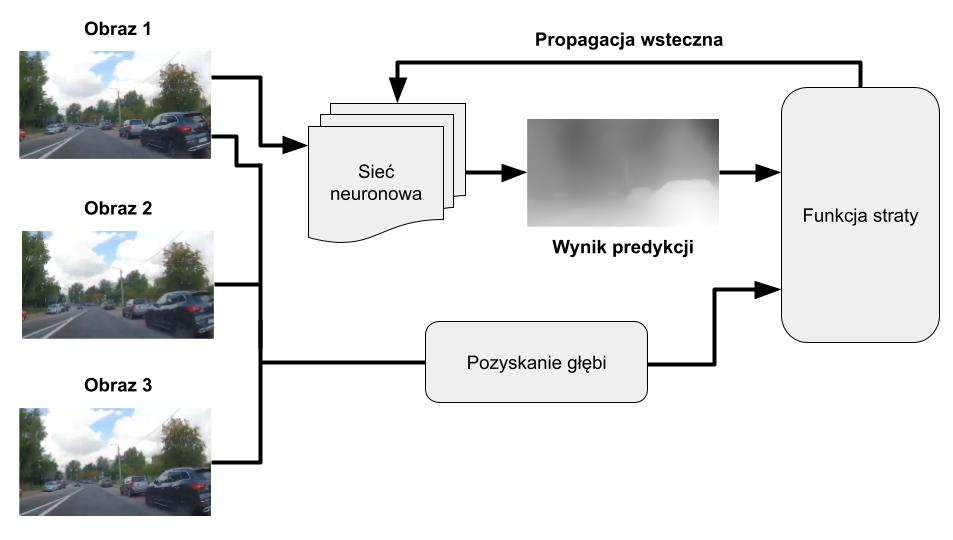
\includegraphics[width=0.80\textwidth]{3.jpg}
    \caption{Schemat przykładowego uczenia nienadzorowanego. Wejścia stanowią trzy kadry z nagrania RGB a wynikiem jest predykcja mapy głębi.}
    \label{fig:uczenie-nienadzorowane}
\end{figure}

\subsection{Uczenie częściowo nadzorowane}
Sposobem łączącym dwa poprzednio przedstawione jest uczenie częściowo nadzorowane. Metoda ta wykorzystuje w procesie uczenia zarówno dane etykietowane jak i nieoznaczone. Głównymi zaletami stosowania tego sposobu są
\begin{itemize}
\item poprawa wydajności algorytmu - ze względu na wykorzystanie większej ilości danych,
\item zmniejszenie kosztów pozyskania danych etykietowanych przy jednoczesnym zachowaniu zadowalających rezultatów,
\item zwiększenie elastyczności modelu ze względu na brak uzależnienia od wyłącznie danych oznaczonych.
\end{itemize}

\vspace{1cm}
Poniższy schemat umieszczony na rys. \ref{fig:podsumowanie-uczenia} przedstawia ogólne podsumowanie paradygmatów uczenia algorytmów.
\begin{figure}[H]
    \centering
    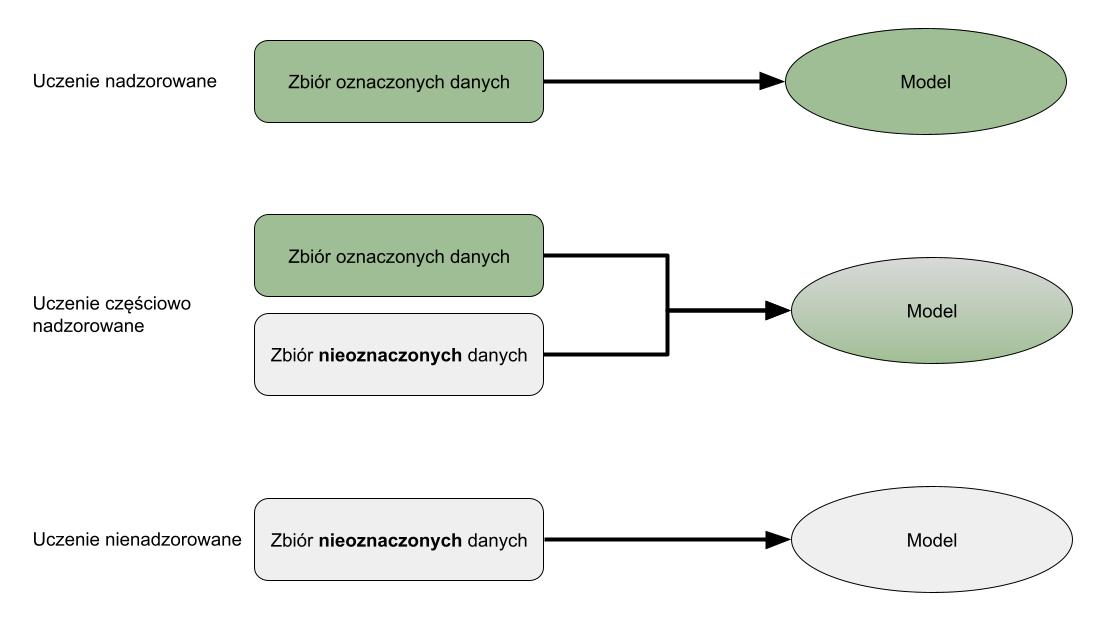
\includegraphics[width=1\textwidth]{4.jpg}
    \caption{Schemat podsumowujący paradygmaty uczenia algorytmów.}
    \label{fig:podsumowanie-uczenia}
\end{figure}

\section{Modele sieci neuronowych w algorytmach percepcji głębi}
Ważnym etapem implementacji algorytmu percepcji głębi jest konstrukcja architektury sieci neuronowej modelu. Ma ona szczególny wpływ na wydajność i skuteczność wynikowego algorytmu. Ten podrozdział zawiera opis dwóch przeważnie wykorzystywanych w dziedzinie percepcji głębi modeli sieci neuronowych.
\subsection{Konwolucyjne sieci neuronowe}
Zaproponowane przez Kunihiko Fukushimę w 1980 r. \cite{fukushima1980} konwolucyjne sieci neuronowe są niewątpliwym kamieniem milowym w komputerowym przetwarzaniu obrazów. Charakteryzuje je zdolność upraszczania obrazu do postaci znacznie łatwiejszej do przetworzenia przez komputer, bez poświęcenia jakości wnioskowania. Podstawowym elementem takich sieci jest warstwa splotowa, w której dochodzi do mnożenia matryc stanowiących dane wejściowe i jądro. Wynikiem mnożenia jest mapa wyodrębnionych cech wejściowego obrazu. Poprawnie przedstawia to poniższa grafika \ref{fig:warstwa-konwolucyjna} oraz \ref{fig:warstwa-konwolucyjna-arch}. W przypadku takiego modelu nauczanie sieci polega między innymi na ustanowieniu odpowiednich wag jądra.
\begin{figure}[H]
    \centering
    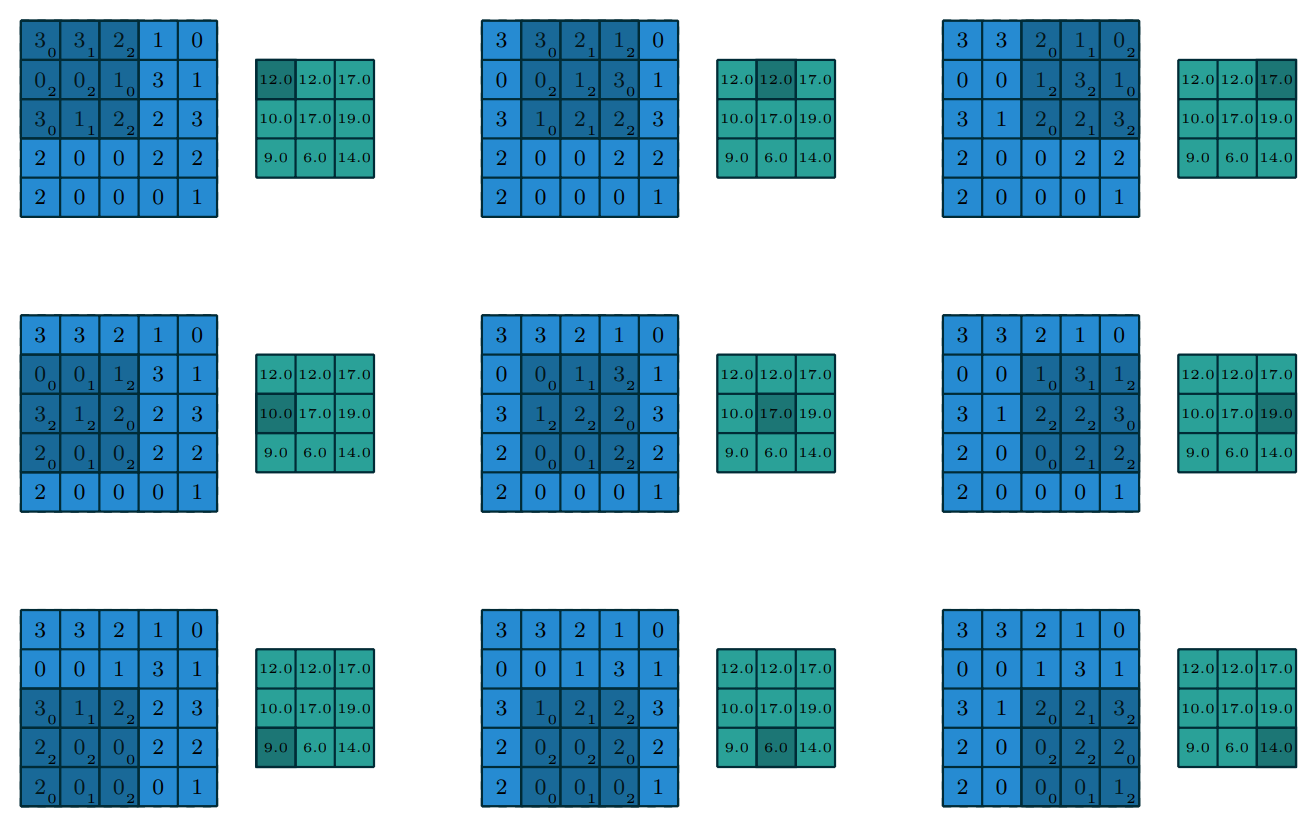
\includegraphics[width=0.9\textwidth]{5.jpg}
    \caption{Przykład działania warstwy konwolucyjnej z jądrem o rozmiarze 3x3. Źródło: \cite{dumoulin2018}}
    \label{fig:warstwa-konwolucyjna}
\end{figure}
\begin{figure}[H]
    \centering
    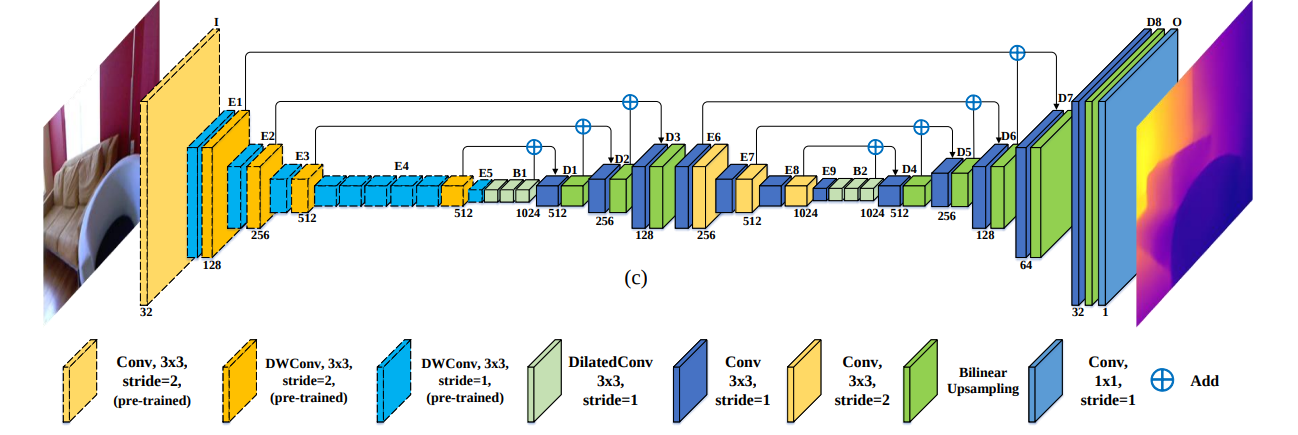
\includegraphics[width=0.9\textwidth]{6.jpg}
    \caption{Przykład architektury sieci konwolucyjnej użytej w celu rozpoznania głębi obrazu. Źródło: \cite{dong2022}}
    \label{fig:warstwa-konwolucyjna-arch}
\end{figure}

\subsection{Transformatory}
Zaprezentowane w 2017 r. \cite{vaswani2017} transformatory wykorzystywane były pierwotnie w przetwarzaniu języka naturalnego. Dzięki asynchronicznej charakterystyce przetwarzania sekwencji wejściowej okazały się znacznie szybsze niż dotychczas znane rozwiązania\footnote{Do ówczesnej chwili częściej używane były sieci rekurencyjne.}.

W kontekście wizyjnych algorytmów wykorzystywane są transformatory wizyjne zaproponowane w 2020 r. przez zespół Google Research w \cite{dosovitskiy2020}. Jego schemat poglądowy przedstawia poniższa grafika \ref{fig:schemat-vit}.
\begin{figure}[H]
    \centering
    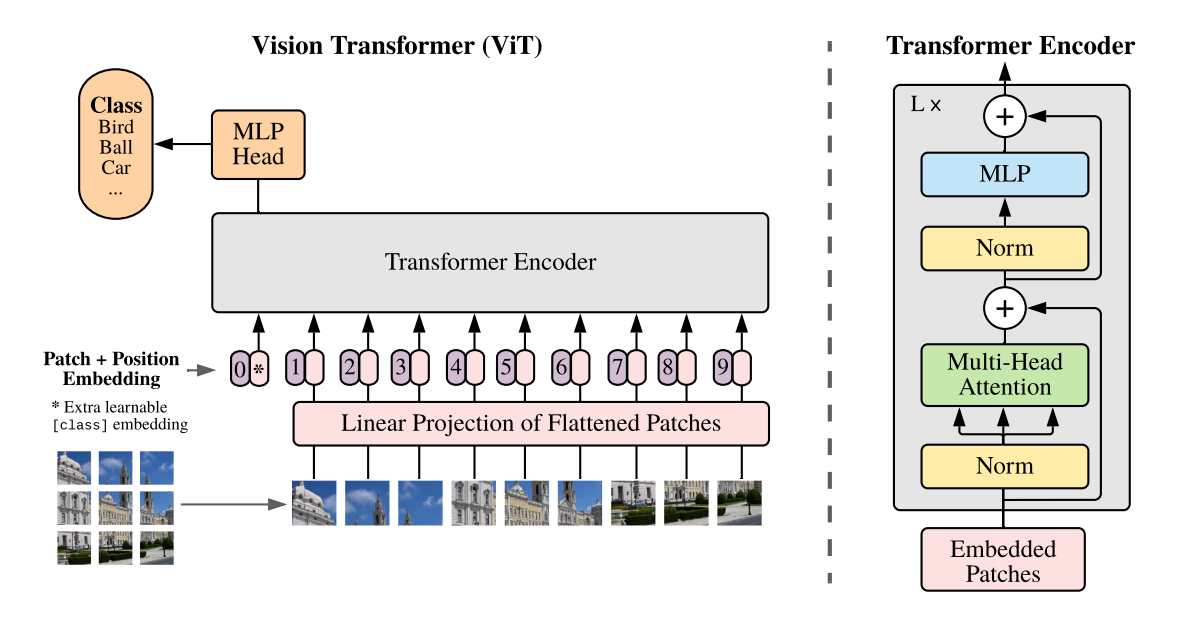
\includegraphics[width=1\textwidth]{7.jpg}
    \caption{Schemat modelu transformatora wizyjnego. Źródło: \cite{dosovitskiy2020}}
    \label{fig:schemat-vit}
\end{figure}
Wizyjny model transformatora nie generalizuje danych tak dobrze jak robi to sieć konwolucyjna, dlatego przy niewielkiej liczbie obrazów uczących nie jest najlepszym wyborem. Jednak przy wykorzystaniu znacznego rozmiaru zestawu obrazów uczących osiągana dokładność najczęściej przewyższa sieci konwolucyjne.